\documentclass{article}

% if you need to pass options to natbib, use, e.g.:
%     \PassOptionsToPackage{numbers, compress}{natbib}
% before loading neurips_2021

% ready for submission
\usepackage{neurips_2021}

% to compile a preprint version, e.g., for submission to arXiv, add add the
% [preprint] option:
%     \usepackage[preprint]{neurips_2021}

% to compile a camera-ready version, add the [final] option, e.g.:
%     \usepackage[final]{neurips_2021}

% to avoid loading the natbib package, add option nonatbib:
%    \usepackage[nonatbib]{neurips_2021}

\usepackage[utf8]{inputenc} % allow utf-8 input
\usepackage[T1]{fontenc}    % use 8-bit T1 fonts
\usepackage{hyperref}       % hyperlinks
\usepackage{url}            % simple URL typesetting
\usepackage{booktabs}       % professional-quality tables
\usepackage{amsfonts}       % blackboard math symbols
\usepackage{nicefrac}       % compact symbols for 1/2, etc.
\usepackage{microtype}      % microtypography
\usepackage{xcolor}         % colors
\usepackage{bm}
\usepackage{amsmath,amssymb}
\usepackage{graphicx}
\usepackage{subfigure}
\bibliographystyle{unsrtnat}

\DeclareMathOperator*{\argmax}{arg\,max}
\DeclareMathOperator*{\argmin}{arg\,min}

\title{Clustering Neural Populations by Poisson Dynamic Factor Model}

% The \author macro works with any number of authors. There are two commands
% used to separate the names and addresses of multiple authors: \And and \AND.
%
% Using \And between authors leaves it to LaTeX to determine where to break the
% lines. Using \AND forces a line break at that point. So, if LaTeX puts 3 of 4
% authors names on the first line, and the last on the second line, try using
% \AND instead of \And before the third author name.

\author{%
	David S.~Hippocampus\thanks{Use footnote for providing further information
		about author (webpage, alternative address)---\emph{not} for acknowledging
		funding agencies.} \\
	Department of Computer Science\\
	Cranberry-Lemon University\\
	Pittsburgh, PA 15213 \\
	\texttt{hippo@cs.cranberry-lemon.edu} \\
	% examples of more authors
	% \And
	% Coauthor \\
	% Affiliation \\
	% Address \\
	% \texttt{email} \\
	% \AND
	% Coauthor \\
	% Affiliation \\
	% Address \\
	% \texttt{email} \\
	% \And
	% Coauthor \\
	% Affiliation \\
	% Address \\
	% \texttt{email} \\
	% \And
	% Coauthor \\
	% Affiliation \\
	% Address \\
	% \texttt{email} \\
}

\begin{document}
	
	\maketitle
	
	\begin{abstract}
	Modern recording techniques allow neuroscientists to study multiple neural populations over extended time periods in a large-scale, and the relationships within and between populations are summarized by low-dimensional latent vectors. When the neural activities are globally nonlinear, using single population analysis is inappropriate. However, defining the populations is usually difficult and  wrong cluster assignments will lead to bias in latent structure inferences. To tackle this challenge, we develop a clustering method based mixture of Poisson dynamic factor model. The number of cluster is treated as a parameter in mixture of finite mixtures (MFM) model, and the posteriors are sampled by a MCMC algorithm. To sample the posteriors efficiently, we approximate the full conditional distribution of latent state by Gaussian and approximate the marginal likelihood by making use of the Poisson-Gamma conjugacy. We further apply our method to neuropixel data (and hippocampus data) for illustration.
	\end{abstract}
	
	\section{Introduction}
	\label{intro}
	\answerTODO{}
	
	\section{Method}
	\label{method}
	
	\subsection{Poisson Dynmic Factor Model}
	Denote the observed spike-count of neuron $i \in \{ 1,\ldots,N\}$ at
	time bin $t \in \{ 1,\ldots,T\}$ as
	$y_{it} \in \mathbb{Z}_{\geq 0}$, and let
	$\bm{y}_{i} =  (y_{i1},\ldots,y_{iT})'$.
	Further, let $z_{i} = j$ denote the cluster indicator of neuron $i$. To facilitate clustering, we re-parametrize the regular Poisson linear dynamical system (PLDS) model \citep{Macke2011} to separate the mean log-firing-rate out. Assume neurons are independently Poisson distributed, conditional on the
	low-dimensional latent state $\bm{x}_{t}^{(j)} \in \mathbb{R}^{p}$ as follows:
	\begin{align*}
		y_{it} &\sim Poi(\lambda_{it})\\
		\log\lambda_{it} &= \mu_t^{(j)} + \bm{c}'_i\bm{x}^{(j)}_t
	\end{align*}
	, with $\bm{c}_i\sim N(\bm{0},\bm{I}_p)$. We further assume the intercept $\mu_t^{(j)}$ and the latent state $\bm{x}^{(j)}_t$ progress linearly with Gaussian noise as
	\begin{align*}
		\mu_1^{(j)} &\sim N(\mu_0, \Sigma_0)\\
		\mu_{t+1}^{(j)} &\sim N(f^{(j)}\mu_t^{(j)} + g^{(j)}, \sigma^{2(j)})\\
		\bm{x}_1^{(j)} &\sim N(\bm{x}_0, \bm{Q}_0)\\
		\bm{x}_{t+1}^{(j)} &\sim N(\bm{A}^{(j)}\bm{x}_t^{(j)} + \bm{b}^{(j)}, \bm{Q}^{(j)})
	\end{align*}
	
	The bias term ($\bm{b}^{(j)}$) in the latent state is constant across time, unlike ind PLDS, which is  $\bm{b}_t^{(j)}$. When the bias term changes across the time, the update order of $\bm{A}^{(j)}$ and $\bm{b}_t^{(j)}$ will influence the results (usually, the $\bm{A}^{(j)}$ is updated first). When ignoring the updating order, the linear dynamics will have infinite solutions. If the $\bm{A}^{(j)}$ is one solution, then $\bm{A}^{*(j)} = \bm{A}^{(j)} + \bm{M}$ and $\bm{b}_t^{*(j)} = \bm{b}_t^{(j)} - \bm{M}\bm{x}^{(j)}_t$ will be another set of solution, for any $\bm{M} \in \mathbb{R}^{p\times p}$. This causes some inconvenience for inference. The same reason for using the time-constant $g^{(j)}$.
	
	If we denote $\bm{\lambda}_{i} =  (\lambda_{i1},\ldots,\lambda_{iT})'$, $\bm{\mu}^{(j)} = (\mu^{(j)}_1,\ldots,\mu^{(j)}_T)'$ and $\bm{X}^{(j)} = (\bm{x}^{(j)}_1,\ldots,\bm{x}^{(j)}_T)'$, the model can be equivalently written as regular Poisson factor model as
	\begin{align*}
		\bm{y}_i &\sim Poi(\bm{\lambda}_i)\\
		\log\bm{\lambda}_i &= \bm{\mu}^{(j)}+ \bm{X}^{(j)}\bm{c}_i 
	\end{align*}

	However, since the condition $T/N \rightarrow 0$ doesn’t hold \citep{Johnstone2009}, the latent state $\bm{X}^{(j)}$ cannot be consistently estimated, and assuming linear dynamics of $\bm{X}^{(j)}$ resolves the problem. Note that when $p>1$, the model is not unique, since $\bm{X}^{*(j)} = \bm{X}^{(j)}\bm{U}$ also satisfies the equation for any orthogonal matrix $\bm{U}$ of order $p$. To ensure the model indefinability, we simply assume $\bm{A}^{(j)}$ and $\bm{Q}^{(j)}$
	are both diagonal for convenience. See more detailed discussions of the constraints in discussion. Overall, denote the cluster-related parameters of cluster $j$ as $\bm{\theta}^{(j)}= \{\bm{\mu}^{(j)}, \bm{X}^{(j)}, f^{(j)}, g^{(j)}, \sigma^{2(j)},\bm{A}^{(j)}, \bm{b}^{(j)}, \bm{Q}^{(j)}\}$ and the spike counts of neuron i is generated by Poisson dynamic factor model (PDFM) as $\bm{Y}_i\sim PDFM(\bm{\theta}^{(z_i)})$, with the prior of $\bm{\theta}^{(j)}$ as $\bm{H}$. The priors for $\{f^{(j)}, g^{(j)}, \sigma^{2(j)},\bm{A}^{(j)}, \bm{b}^{(j)}, \bm{Q}^{(j)}\}$ are regular  normal and inverse-gamma distribution (or multivariate normal and inverse-Wishart when using other non-diagonal constraints).

	The marginal likelihood of neuron i is
	
	$$M_{\bm{\theta}^{(j)}}(\bm{y}_i) = P(\bm{y}_i|\bm{\theta}^{(j)}) = \int P(\bm{y}_i|\bm{\theta}^{(j)}, \bm{c}_i)P(\bm{c}_i)\,d\bm{c}_i$$
	
	The marginal likelihood has no closed form and will be used for clustering. To help with fast clustering, instead of doing the Laplace approximation, we choose to make use of the Poisson-Gamma conjugacy. This approximation was originally used in \citet{El-Sayyad1973} to derive approximate posterior and the same method was applied to derive other approximations in \citet{Chan2009}. This approximation leads to the closed form approximation. By the conditional independency assumption, $M_{\bm{\theta}^{(j)}}(\bm{y}_i)=\prod_{t=1}^{T}P(y_{it}|\bm{\theta}^{(j)})$. Since $\bm{c}_i\sim N(\bm{0},\bm{I}_p)$, $\lambda_{it} = \exp(\mu_t^{(j)} + \bm{c}'_i\bm{x}^{(j)}_t)\sim lognormal(\mu_t^{(j)}, \bm{x}'^{(j)}_t\bm{x}^{(j)}_t)$. Approximate the lognormal distribution by Gamma distribution, s.t. $lognormal(\mu_t^{(j)}, \bm{x}'^{(j)}_t\bm{x}^{(j)}_t) \approx Gamma(a_{it}, b_{it})$ with $a_{it} = (\bm{x}'^{(j)}_t\bm{x}^{(j)}_t)^{-1}$ and $b_{it} = \bm{x}'^{(j)}_t\bm{x}^{(j)}_t\cdot e^{\mu_t^{(j)}}$. Then by Poisson-Gamma conjugacy,
	
	$$
	P(y_{it}|\bm{\theta}^{(j)}) = \int P(y_{it}|\lambda_{it})P(\lambda_{it})\,d\lambda_{it}\approx NB(y_{it}|r_{it}, p_{it})
	$$
	
	, with $r_{it} = a_{it}$ and $p_{it} = 1/(1 + b_{it})$.
	
	Another more general idea is to approximate the log-likelihood by second-order polynomials, with coefficients determined by Chebyshev polynomial approximation \citet{Keeley2019}. However, the approximation doesn’t work well in practice, especially when the neural spike counts have a wide range. When doing the integration, we need to exponentiate the log-likelihood and this will exaggerate the approximation error.
	
	\subsection{Cluster by Mixture of Finite Mixtures Model}
	When the label is unknown, we cluster the neurons by mixture models. In practice, it’s usually impossible to know the number of neural population. One potential method is to do clustering by Dirichlet process mixtures (DPM) model. However, this is conceptually incorrect, since the number of neural populations is finite but unknown. Besides the conceptual incorrectness, using DPM is not easy to integrate the field knowledge about the number of neural populations. Here, we choose to use the mixture of finite mixtures (MFM, \citet{Miller2018}) model as follows
	
	\begin{align*}
		K &\sim p_K &&\text{where}\, p_K \, \text{is a p.m.f. on} \{1,2,\ldots\}\\
		\bm{\pi}=(\pi_1,\ldots,\pi_k) &\sim Dir_k(\gamma, \ldots,\gamma) &&\text{given} K=k\\
		Z_1,\ldots,Z_n&\stackrel{i.i.d.}{\sim}\pi &&\text{given} \pi\\
		\bm{\theta}_1,\ldots,\bm{\theta}_k&\stackrel{i.i.d.}{\sim}\bm{H} &&\text{given} K=k\\
		\bm{Y}_i = (y_{i1},\ldots,y_{iT})' &\sim SSFM(\bm{\theta}^{(z_i)}) &&\text{independently for}\, i=1,\ldots,N, \text{given}\, \bm{\theta}_{1:K}\, \text{and}\, Z_{1:N}
	\end{align*}
	
	Besides the conceptual correctness, using MFM model allows us integrate the prior knowledge easily. Moreover, compared to DPM, MFM has some better properties for clustering, for example, MFM posterior on number of cluster is more concentrated and consistent, and MFM tend to give clusters size at the same order of magnitude while DPM may lead to a few large clusters and many small clusters. See \cite{Miller2018} for detailed discussion. 
	
	\subsection{Inference}
	
	In this paper, we choose to do inference by MCMC. Because of the Poisson likelihood, the latent state $\bm{X}^{(j)}$has no closed full conditional distribution. We can sample the posterior by particle MCMC directly, but this can be slow. However, due to the Markovian structure of the model, the conditional log-posterior is concave and its Hessian is block-tridiagonal. Thus, we can do the global Laplace approximation efficiently in $\mathcal{O}(T)$ \citep{Paninski2010}.The cluster index and number of cluster are sampled by the analog of partition-based algorithm in DPM \citep{Neal2000}. See details of the MCMC update in the Appendix.
	
	In practice, using variational Bayes (VB) instead of MCMC may be more favorable. The PLDS can be updated by variational EM. Using the stick-breaking representation of MFM model, we can do VB easily similar to \citet{Blei2006}. However, checking by the “gold standard” MCMC before doing VB is always a good choice.
	
	For the dimensionality $p$ of of the latent state, we can treat it as a parameter and sample the posterior by RJMCMC as in \citet{Lopes2004} or borrow the idea of adaptive Gibbs sampling with shrinkage prior \citep{Bhattacharya2011}. Here, we simply pre-set the $p$ or select the optimized value by the cross-validation, which can be easily conducted when switching to the deterministic algorithm in the future. 
	
	\section{Simulations}
	\label{sim}
	
	\subsection{Model Global Non-linearity by Clustering}
	There were a rich research results for single PLDS model, but it provides only a global linear model to represent the data in a lower dimensional subspace, which makes the application scope limited. When the input space is nonhomogeneous, a large dimension of latent state is needed and this may lead to the overfitting and poor performance. Mixture of PLDS/ PDFM models allow us to partition the input space into clusters and can therefore capture global nonlinearity by combining local linear models.
	
	To show the connection between the proposed model and PLDS parametrization, we simulate the data using the PLDS model, although these two are equivalent after some algebra. Denote the common PLDS model as $\log \lambda_i = \delta_i\bm{1}_T + \bm{G}^{(j)}\bm{d}_i$, where $d_i\in \mathbb{R}^q$. In PLDS parametrization, the latent state has one more dimension, i.e. $p=q+1$.
	
	We first simulated three neural populations, with 10 neurons in each. We set $q=2$ for each cluster and the recording length is T=1000. The $\delta_i = 1$ for $i=1,\ldots, 10$ and is $0$ for the remaining neurons. The $\bm{G}^{(j)}$ is $0.1(1,\ldots,10)'\otimes\bm{1}'_2 + \bm{1}_{10}\otimes(-1, 2)$ to set up a gradient for the loading in each cluster and to differ the contribution of two latent vectors. We allow $\bm{A}^{(j)}$ be non-diagonal and possible interactions between clusters, which is used in single population PLDS model. The diagonal element is generated from $N(0.92, 0.1^2)$. The bias terms are $\bm{b}^{(j)}$ is $10^{-3}\bm{1}_2$ for the first 2 clusters and $10^{-4}\bm{1}_2$ for the last cluster. The $\bm{Q}^{(j)}$ are $10^{-3}\bm{I}_2$, $10^{-4}\bm{I}_2$ and $10^{-5}\bm{I}_2$.
	
	The Figure \ref{fig:1a} shows the trace plot for the log-likelihood per spike, up to 10,000 iterations. The plot shows (Figure \ref{fig:1b}) that the convergence achieved after several steps. Therefore, we show the results by averaging iteration 500 to 1000. Figure \ref{fig:1c} shows the posterior mean of the mean firing rate, while Figure \ref{fig:1d} shows the fitted latent state. The latent vectors are transformed to PLDS parametrization for comparison. Notice that the PLDS parametrization also doesn't have the unique solution, we let $\bm{G}^{(j)}$ has mean zeros columns and is orthogonal.
	
	Then we held out $1/4$ and $1/2$ data as test set in a “speckled” pattern, i.e. randomly select subset of data for each neuron as held-out dataset. The "speckled" cross-validation was previously used in \cite{Williams2020}. We then fit the model with and without clusters, keeping the same latent dimension, i.e. (1) 3 clusters with $p=1$ for each and (2) 1 cluster with $p=2\cdot 3 - 1 = 5$. The procedure is replicated for 100 times for two proportions, and the difference of held-out likelihood per spike between 2 fittings are shown in Figure \ref{fig:1e}. The difference between (1) and (2) are always positive, and this shows doing the mixture of PDFM performs better than single PDFM. Moreover, as the proportion of training decrease (less data), the benefit of clustering becomes more significant. This suggests that doing clustering is necessary.
	
	\begin{figure}[h!]
		\centering
		\subfigure[Trace plot of  log-likelihood per spike]{\label{fig:1a}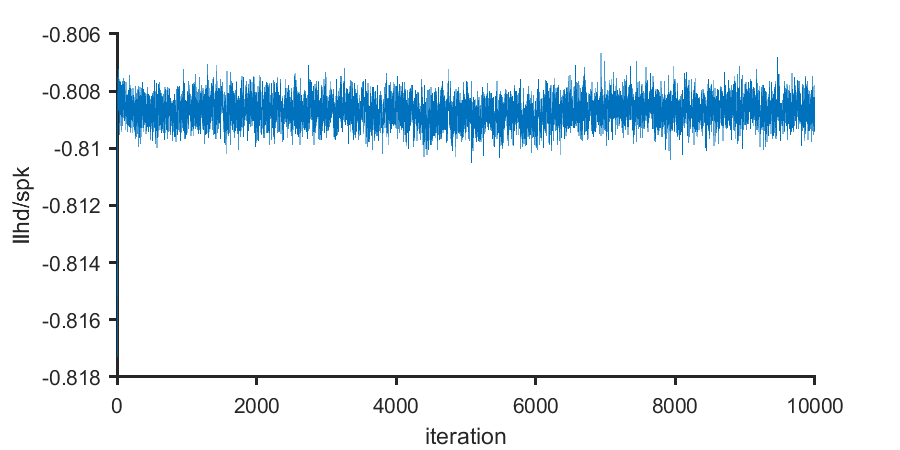
\includegraphics[width=0.5\textwidth]{2_llhd1.png}}%
		\subfigure[Trace plot of  log-likelihood per spike, truncated (1000)]{\label{fig:1b}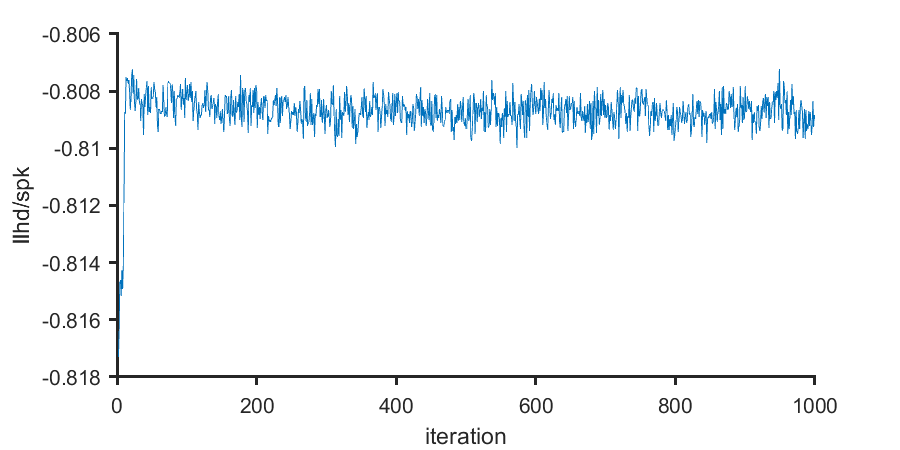
\includegraphics[width=0.5\textwidth]{3_llhd2.png}}%
		
		\subfigure[true vs. fitted firing rate]{\label{fig:1c}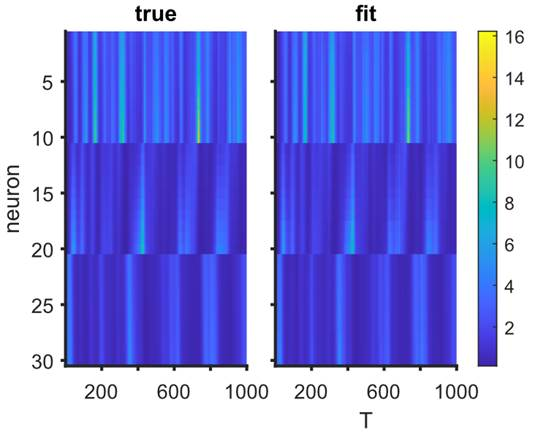
\includegraphics[width=0.5\textwidth]{image001.jpg}}%
		\subfigure[true vs. fitted latent vectors]{\label{fig:1d}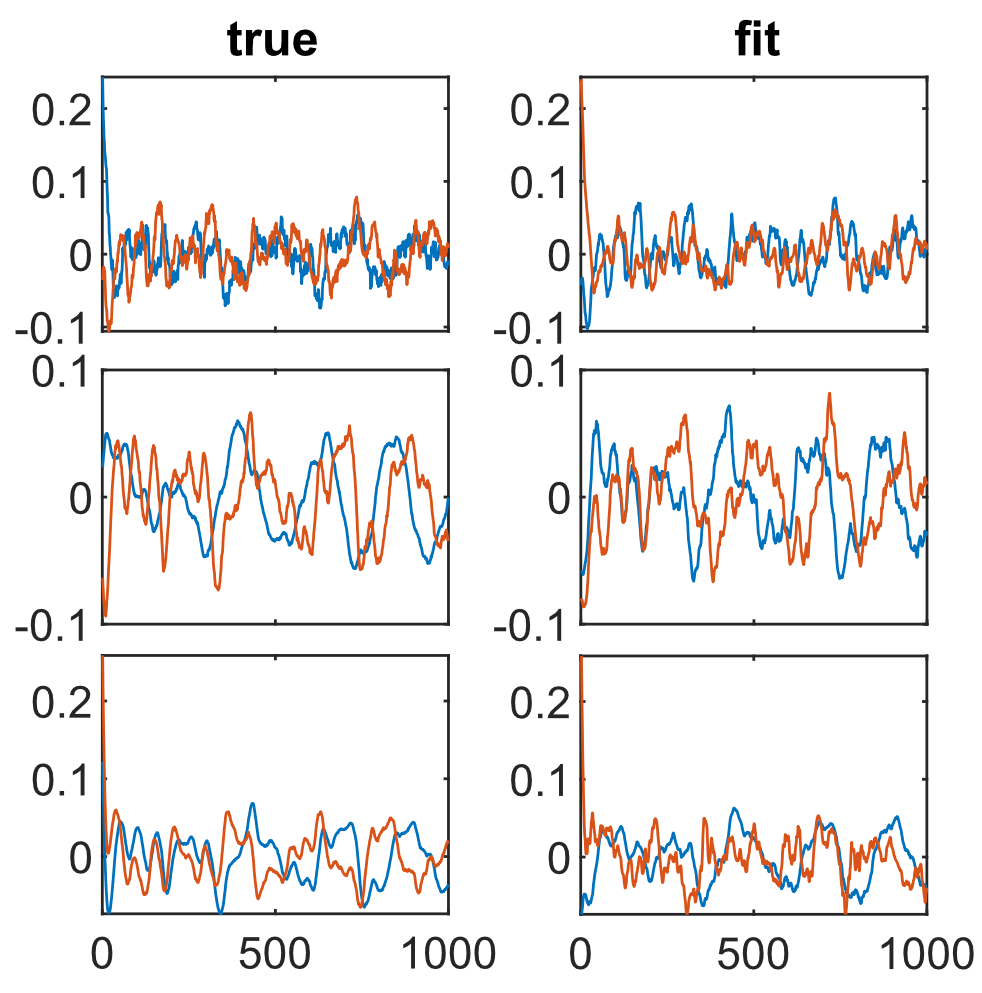
\includegraphics[width=0.5\textwidth]{LF.png}}%
		
		\subfigure[cross-validation: clustered vs. single population]{\label{fig:1e}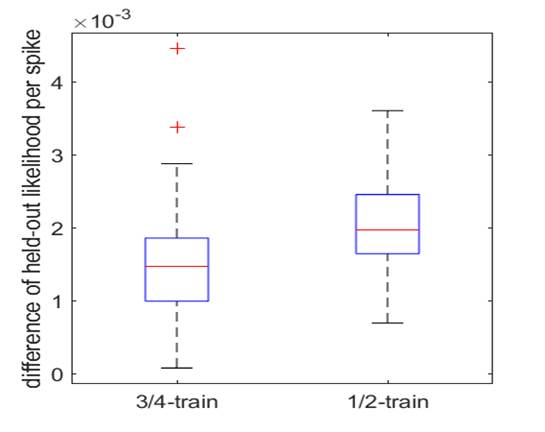
\includegraphics[width=0.5\textwidth]{image003.jpg}}%
		\subfigure[trace plot for non-labeled case]{\label{fig:1f}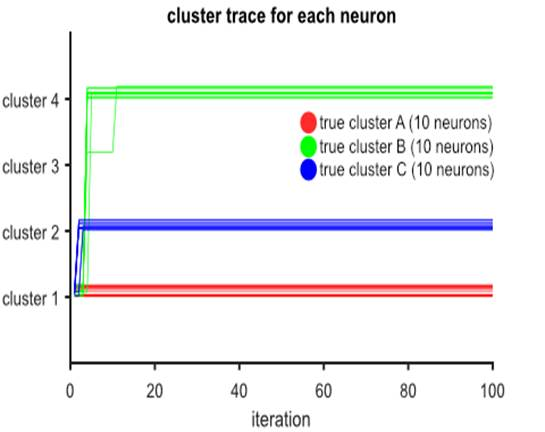
\includegraphics[width=0.5\textwidth]{image004.jpg}}%
		\caption{Simple case}
	\end{figure}
	
	\subsubsection{Clustering}
	Then use the same setting, we remove the label and use the mixture model to do the clustering by MFM. The prior of the cluster number is $K\sim Geometric(0.2)$. Figure \ref{fig:1f} shows the trace of label $z_i$ for each neuron for the first 100 iterations.
	
	\begin{figure}[h!]
		\centering
		\subfigure[Firing rate]{\label{fig:2a}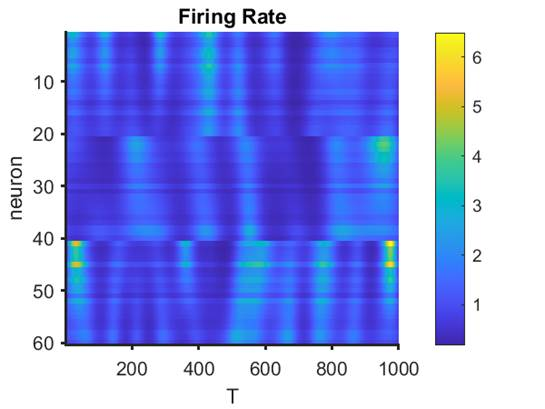
\includegraphics[width=0.4\textwidth]{image005.jpg}}%
		\subfigure[trace plot for cluster number]{\label{fig:2b}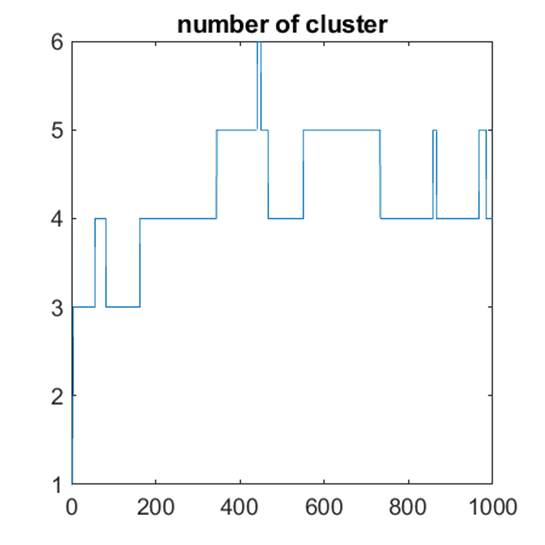
\includegraphics[width=0.4\textwidth]{image006.jpg}}%
		\subfigure[similarity matrix]{\label{fig:2c}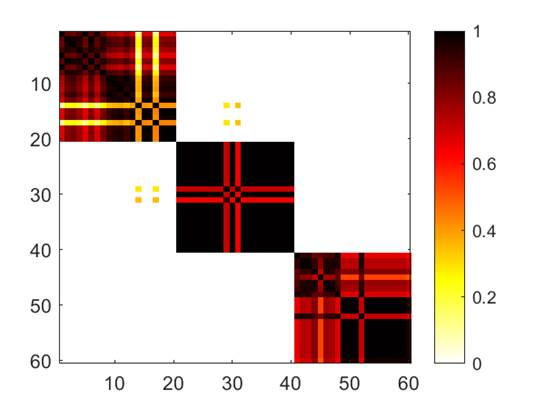
\includegraphics[width=0.4\textwidth]{image007.jpg}}%
		\caption{More complicated case: more variety of amplitude \& weaker signal}
	\end{figure}
	
	In this toy simulation example, the signal is strong and the spiking amplitudes of neurons in each population are similar. This might be too simplified for real situation. In practice, the neural activity is usually sparse and can be recorded in high resolution. Moreover, the spiking amplitudes for neuron in one nominated population vary a lot, and hence may form a few subpopulations. Therefore, we then simulate another more realistic example. In this simulation, there are 3 clusters and the dimension of latent state is $p=1$ for each. However, there are 20 neurons with wider range but smaller value of loading $c_i$, corresponding to potential subpopulations and weak signal. The simulated firing rate is shown in Figure \ref{fig:2a}. The trace plot of number of cluster (Figure \ref{fig:2b}) shows that the model tend to further split some clusters into sub-population, based on the spiking amplitude. This is more clearly shown in the posterior similarity matrix ((Figure \ref{fig:2c}), averaging from iteration 500 to 1000. In similarity matrix, the entry $(i,j)$ is the posterior probability that data points $i$ and $j$ belong to the same cluster. The rows and columns are ordered according to the ground truth. The similarity matrix shows that the model tend to split cluster 1 and 3 into two sub-clusters.
	
	\section{Application}
	\label{app}
	
	\subsection{Neuropixels data}
	\answerTODO{}: brief introduction of Neuropixels dataset.
	
	The Neuropixels dataset contains recording of neural activities in different brain regions of mouse. Here, we only consider neurons with SNR > 3 and the spiking counts > 1000. Then, we first use the recording activity from Lateral posterior nucleus of the thalamus (LP, 20 neurons), anteromedial visual area (VISam, 12 neurons) and ventral posteromedial nucleus of the thalamus (VPM, 14 neurons) during the spontaneous period. The bin size is 0.1s and truncate the data up to 1000 steps (100s recording) for convenience. 
	
	Figure \ref{fig:3a} shows the spiking counts of these 46 neurons. Here we first fit model using all data, with $p=1$ and $K\sim Geometric(0.3)$. For the number of clusters, Figure \ref{fig:3b} shows the trace plot for the first 5000 iterations. All the following results are from averaging samples from iteration 2500 to 5000. The Figure \ref{fig:3c} shows the histogram of the posterior samples. These plots show that these neurons are quite non-homogeneous and they tend to form many sub-populations. These 3 nominated populations by anatomy tend to form around 10 (sub)-clusters.
	
	The Figure \ref{fig:3d} and Figure \ref{fig:3e} show the trace of log-likelihood per spike. The fitted mean firing rate is shown in Figure \ref{fig:3f}. When investigating the similarity matrix in Figure \ref{fig:3g} (sorted according to the anatomical population, such that 1-20 are LP, 21-32 are VISam and 33-46 are VPM), there are several subpopulations in each anatomical cluster. Generally, the clustering results are consistent with the anatomical assignment, although there are some tiny confusions between VISam and VPM.
	
	However, this is not the case when the mouse is in the experiment. We choose the same set of neurons but use recordings when the mouse are watching drift gratings. The Figure \ref{fig:3h} shows the trace plot of cluster number. The Figure \ref{fig:3i} and Figure \ref{fig:3j} show the fitted firing rate and similarity matrix, again averaging from iteration 2500 to 5000.
	
	When comparing the observed spiking activities, it's fairly hard to see differences when the mouse is exposed to the stimuli and not. However, the posterior similarity matrix in the experiment shows that there's more confusion between LP and VISam, compared to the spontaneous response. This suggests that the functional connection pattern between neurons in different areas when the stimuli are changed.
	
	\textcolor{red}{\textbf{I tried to held-out half of the data in a speckled pattern and fit the model with clustering on and off (single population). The dimension is selected by held-out likelihood, which is p=1 for clustering on and p=2 for single population analysis. The trace plots of the held-out log-likelihood per spike (starting from iteration 2) shows that doing clustering doesn’t improve things (although they are very close)… Maybe because “turning clustering on” introduce too much variance… The benefit of clustering will pop out if we use the deterministic algorithm, such as VB mentioned.}}
	
	\begin{figure}[h!]
		\centering
		\subfigure[spontaneous: spike counts]{\label{fig:3a}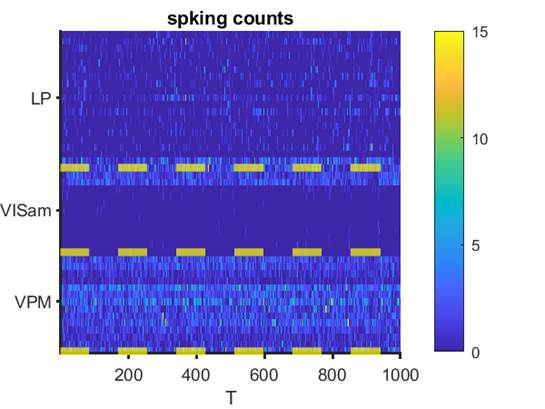
\includegraphics[width=0.5\textwidth]{image008.jpg}}%
		\subfigure[spontaneous: cluster number trace]{\label{fig:3b}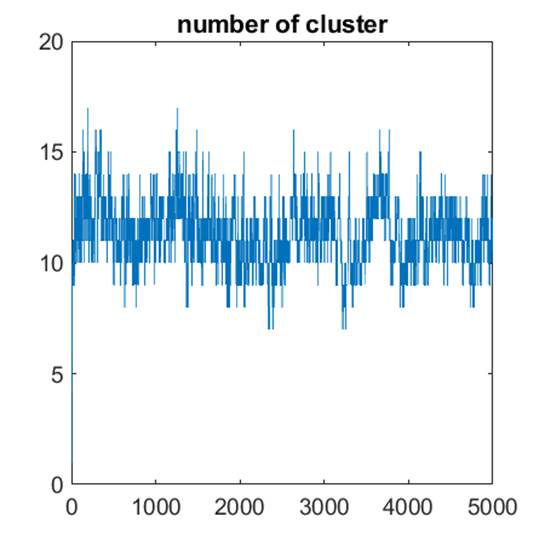
\includegraphics[width=0.35\textwidth]{image009.jpg}}%
		\subfigure[spontaneous: cluster number histogram]{\label{fig:3c}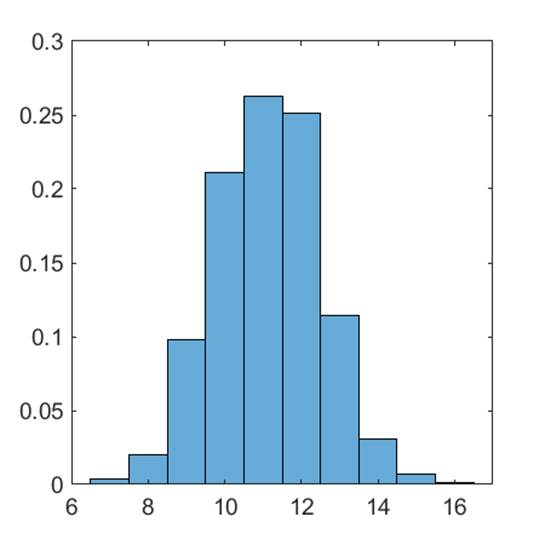
\includegraphics[width=0.35\textwidth]{image010.jpg}}%
		
		\subfigure[spontaneous: llhd/spk trace]{\label{fig:3d}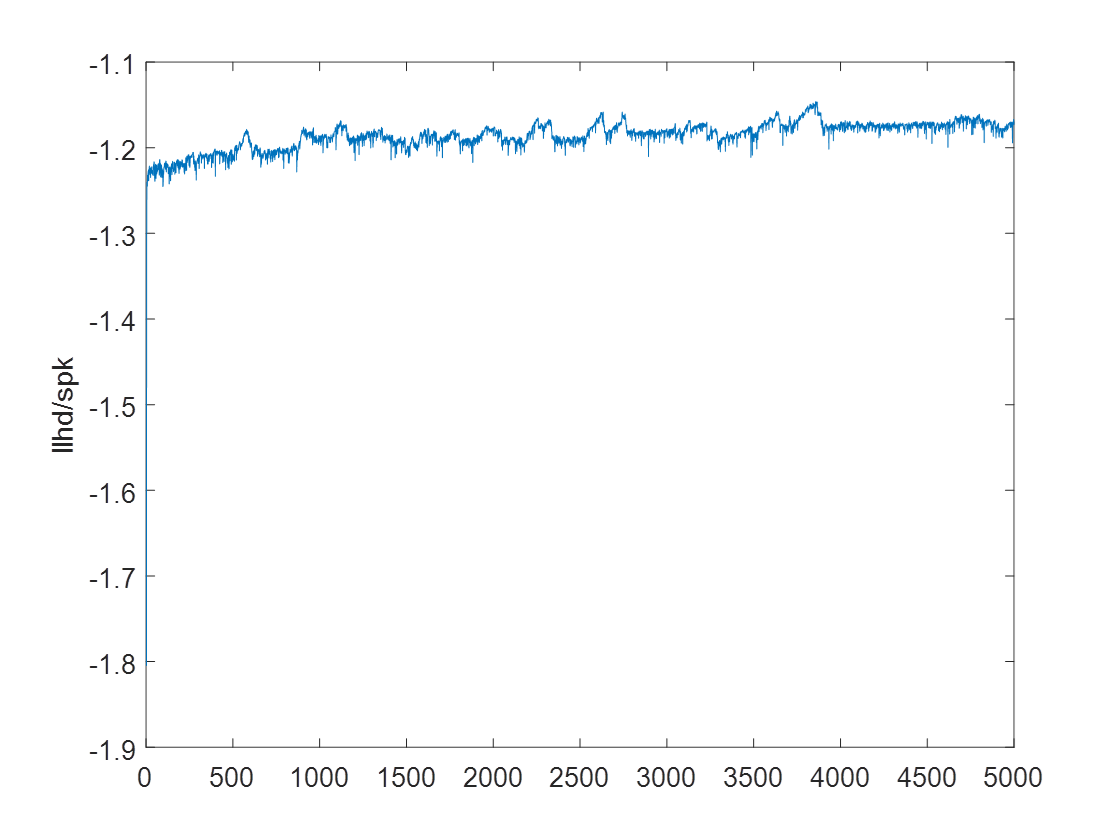
\includegraphics[width=0.3\textwidth]{image001.png}}%
		\subfigure[spontaneous: llhd/spk trace, truncated]{\label{fig:3e}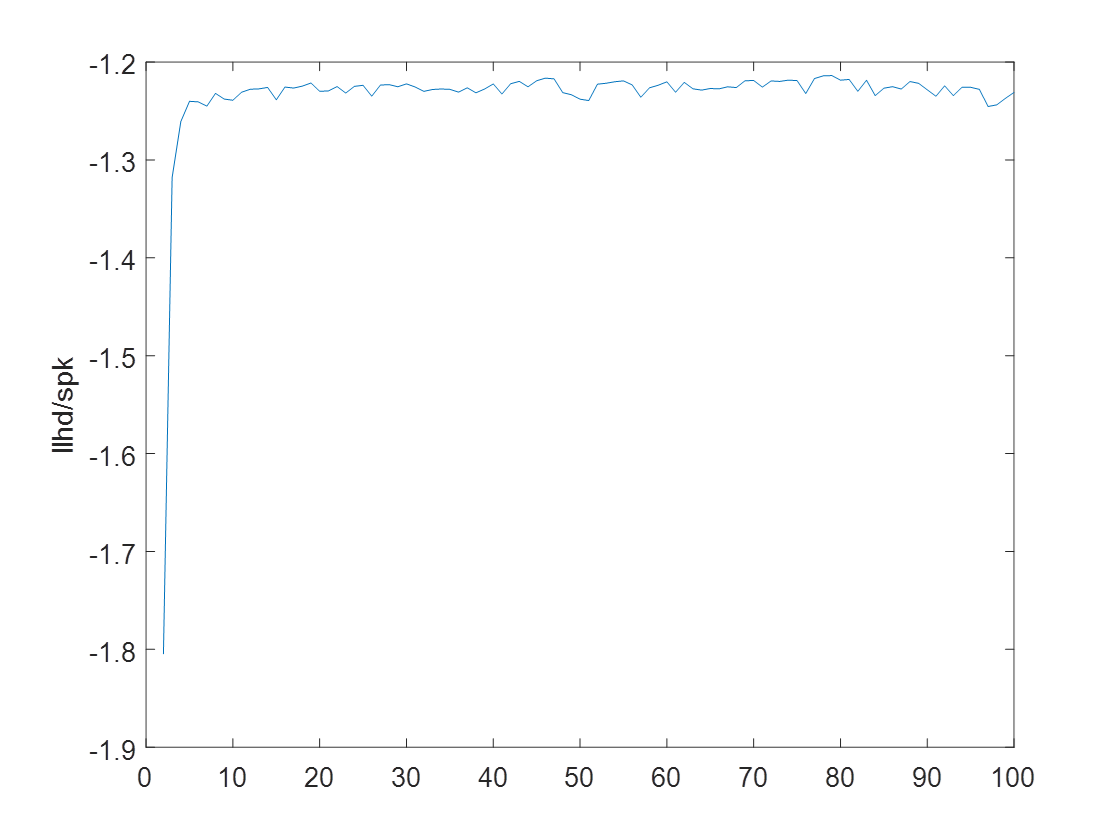
\includegraphics[width=0.3\textwidth]{image002.png}}%
		\subfigure[spontaneous: true vs. fitted firing rate]{\label{fig:3f}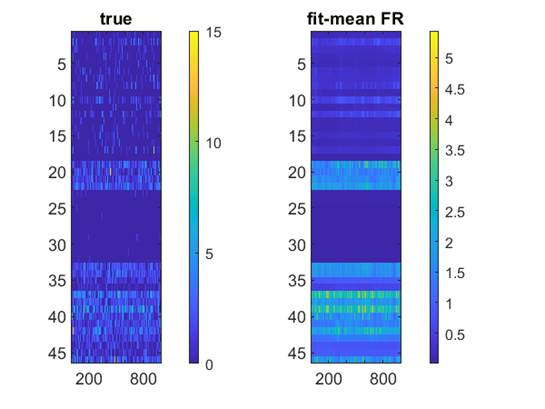
\includegraphics[width=0.3\textwidth]{image011.jpg}}%
		\subfigure[spontaneous: similarity matrix]{\label{fig:3g}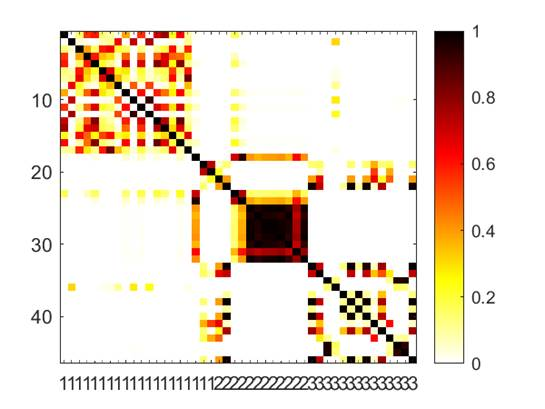
\includegraphics[width=0.3\textwidth]{image012.jpg}}%
		
		\subfigure[drift-grating: cluster number trace]{\label{fig:3h}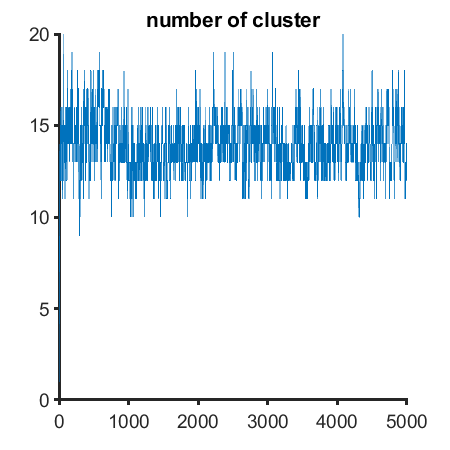
\includegraphics[width=0.4\textwidth]{12_numTrace.png}}%
		\subfigure[drift-grating: true vs. fitted firing rate]{\label{fig:3i}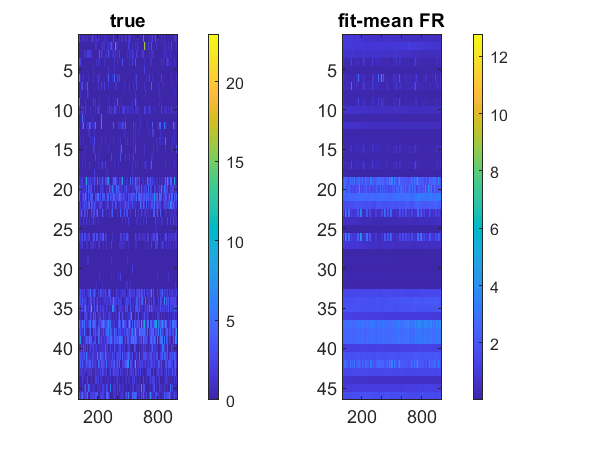
\includegraphics[width=0.4\textwidth]{16_fitFR.png}}%
		\subfigure[drift-grating: similarity matrix]{\label{fig:3j}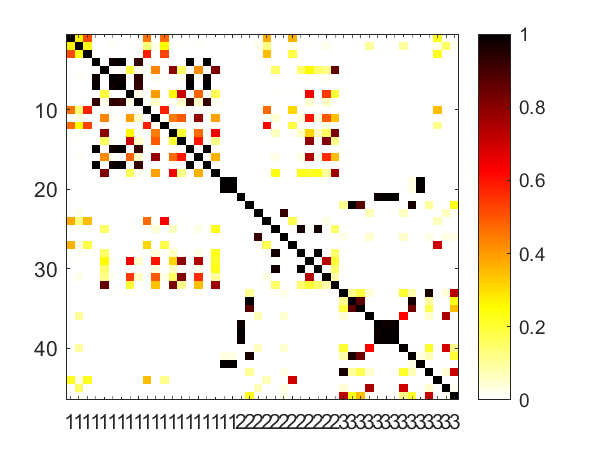
\includegraphics[width=0.4\textwidth]{14_simPixel.png}}%
		\caption{Neuropixel}
	\end{figure}
	
	\subsection{Hippocampus data}
	
	\textcolor{red}{\textbf{I prefer just give one application.} Because 1) there's a page limit (9 pages excluding ref \& appendix in 2021, and now it seems we will exceed the limit), and 2) the V1 data is enough to illustrate the idea If we really need to add the second example, we should tell the story in another angle}.
	
	\section{Discussion}
	
	As mentioned above, the factor model doesn’t have unique solution. Although this issue had been thoroughly discussed in statistics [reference], it has been ignored in some neuroscience research. Since the (P)LDS related model are usually fitted by deterministic algorithms such as variants of EM, the issue is kind of hard to detect. And because of the ignorance, there are some problematic comments on linear dynamics $\bm{A}$ and $\bm{Q}$. When using the variants of factor model, e.g. (P)LDS and GPFA, we should only focus on the “shape” of latent state but not the specific values of them.
	
	In this paper, to ensure the unique solution, we put the diagonal constraints in $\bm{A}^{(j)}$ and $\bm{Q}^{(j)}$ are used for convenience. However, only constraining on $p(p-1)/2$ s enough [reference]. Since we the label is unknown and will be switched when doing clustering, it’s inappropriate and convenient to put constraint on $\bm{c}_i$. Therefore, we instead treat $\bm{X}^{(j)}$ as the "loading" and can put constraints on it. In traditional Gaussian factor model, there are two equivalent types of constraints: (1) diagonal constraint: $\bm{X}'^{(j)}\bm{X}^{(j)}$ is diagonal; (2) block lower triangular constraint \citep{Fokoue2003}: The first $p$ rows of $\bm{X}^{(j)}$ is lower triagular and the diagonal elements are positive. Since we assume $\bm{X}^{(j)}$ has linear progression, using the diagonal $\bm{X}'^{(j)}\bm{X}^{(j)}$ constraint is more appropriate. This constraint can be easily achieved when conducting deterministic optimization algorithms (e.g. the VB mentioned in “method-inference” section). This can also be done in MCMC, by turning off the reflection of the projection (e.g. let the diagonal elements in the projection matrix be positive). Using diagonal $\bm{X}'^{(j)}\bm{X}^{(j)}$  leads to similar results.
	
	Moreover, the idea of doing clustering by mixture model can be extended beyond the Poisson distribution. We can further include other information, such as, the dispersion information by assuming negative-binomial distributed or even Conway-Maxwell-Poisson distributed neural spikes [reference to our paper in CMP]. This further information can be used for more detailed clustering, by expanding the state space.
	
	\section*{Acknowledgments}
	
	\section*{Broader Impact}
	
	\newpage
	{
		\small
		\bibliography{MyCollection}
	}
	
	%%%%%%%%%%%%%%%%%%%%%%%%%%%%%%%%%%%%%%%%%%%%%%%%%%%%%%%%%%%%
	
	\appendix
	
	\section{Appendix}
	
	\subsection{MCMC updates}
	The posteriors are sampled by a Gibbs sampler, the full conditional distributions, if available, are shown as follows:
	
	\underline{\textit{Update $x_t^{(j)}$ and $\mu_t^{(j)}$}}:
	Let the $t^{\text{th}}$ column observation and firing rate of the $j^{\text{th}}$ cluster be $\widetilde{\bm{y}}_t = vec\left(\{y_{it}^{(j)}|z_i = j\}\right)$ and $\widetilde{\bm{\lambda}}_t^{(j)} = vec\left(\{\lambda_{it}|z_i = j\}\right)$. The number of neurons in cluster $j$ is $n_j=\left|\{i:z_i = j\}\right|$. The corresponding loading for these $n_j$ neurons is $\bm{C}^{(j)}\in\mathbb{R}^{n_j\times p}$, such that $\log \widetilde{\bm{\lambda}}_t^{(j)} = \mu_t^{(j)}\bm{1}_{n_j} + \bm{C}^{(j)}\bm{x}_t^{(j)} = \left(\bm{1}_{n_j}, \bm{C}^{(j)} \right)\cdot \left(\mu_t^{(j)}, \bm{x}_t^{'(j)}\right)'$. Denote $\bm{\widetilde{C}}^{(j)} = \left(\bm{1}_{n_j}, \bm{C}^{(j)} \right)$, $\bm{\widetilde{x}}_t^{(j)} = \left(\mu_t^{(j)}, \bm{x}_t^{'(j)}\right)'$, $\bm{\widetilde{x}}^{(j)} = \left(\bm{\widetilde{x}}_1^{'(j)},\ldots,\bm{\widetilde{x}}_T^{'(j)}\right)'$, $\widetilde{\bm{A}}^{(j)} = diag(f^{(j)}, \bm{A}^{(j)})$, $\widetilde{\bm{b}}^{(j)} = \left(g^{(j)}, \bm{b}^{'(j)}\right)'$ and $\widetilde{\bm{Q}}^{(j)} = diag(\sigma^{2(j)}, \bm{Q}^{(j)})$. The full conditional distribution $P(\bm{\widetilde{x}}^{(j)}|\ldots) = P(\bm{\widetilde{x}}^{(j)}|\{\widetilde{\bm{y}}_t\}_{t=1}^T, \bm{\widetilde{C}}^{(j)}, \widetilde{\bm{A}}^{(j)}, \widetilde{\bm{b}}^{(j)}, \widetilde{\bm{Q}}^{(j)})$ is approximated by a global Laplace approximation, i.e. $P(\bm{\widetilde{x}}^{(j)}|\ldots) \approx  N_{(p+1)T}(\bm{\widetilde{x}}^{(j)} | \bm{\mu}_{\widetilde{\bm{x}}^{(j)}}, \bm{\Sigma}_{\widetilde{\bm{x}}^{(j)}})$, with $\bm{\mu}_{\widetilde{\bm{x}}^{(j)}} = \argmax_{\widetilde{\bm{x}}^{(j)}}P(\bm{\widetilde{x}}^{(j)}|\ldots)$ and $\bm{\Sigma}_{\widetilde{\bm{x}}^{(j)}}) = -\left(\nabla\nabla \log P(\bm{\widetilde{x}}^{(j)}|\ldots)\right |_{\bm{\widetilde{x}}^{(j)} = \bm{\mu}_{\widetilde{\bm{x}}^{(j)}}} )^{-1}$. The log full conditional distribution $h(\bm{\widetilde{x}}^{(j)}) = \log P(\bm{\widetilde{x}}^{(j)}|\ldots)$ is given by:
	\begin{align*}
		h &= \text{const} + \sum_{t=1}^{T} \left(\widetilde{\bm{y}}'_t\bm{\widetilde{C}}^{(j)}\bm{\widetilde{x}}_t^{(j)} - \widetilde{\bm{\lambda}}_t\right)
		- \frac{1}{2}(\bm{\widetilde{x}}_1^{(j)}  - \bm{\widetilde{x}}_0^{(j)})'\bm{\widetilde{\bm{Q}}}^{(j)}_0(\bm{\widetilde{x}}_1^{(j)}  - \bm{\widetilde{x}}_0^{(j)})\\ 
		&-\sum_{t=2}^{T}\frac{1}{2}(\bm{\widetilde{x}}_t^{(j)}  - \widetilde{\bm{A}}^{(j)}\bm{\widetilde{x}}_{t-1}^{(j)} - \widetilde{\bm{b}}^{(j)})'\bm{\widetilde{\bm{Q}}}^{(j)}(\bm{\widetilde{x}}_t^{(j)}  - \widetilde{\bm{A}}^{(j)}\bm{\widetilde{x}}_{t-1}^{(j)} - \widetilde{\bm{b}}^{(j)})
	\end{align*}
	, where "const" represents the constant. The $h(\bm{\widetilde{x}}^{(j)})$ is concave and hence unimodal, and the Markovian structure of the latent dynamics, and hence the tri-block-diagonal Hessian, makes it possible to compute a Newton update in $\mathcal{O}(T)$ \citep{Paninski2010}. The same technique is used in the E-step for PLDS model \citep{Macke2011}.
	
	To facilitate convergence, we use a smoothing estimate with local Gaussian approximation as a "warm start". The forward filtering for a dynamic Poisson model has been previously described in \cite{Eden2004}. Because the approximated filtering estimates are Gaussian distributed, we can further find the smoothing estimates using a backward pass as in \cite{RAUCH1965}.
	
	\underline{\textit{Update $\bm{c}_i$}}: 
	When writing the observation mapping in matrix form,
	$\log\bm{\lambda}_i = \bm{\mu}^{(j)}+ \bm{X}^{(j)}\bm{c}_i$, the update of $\bm{c}_i$ reduces to a regular Poisson regression problem, given $\bm{\mu}^{(j)}$ and $\bm{X}^{(j)}$ are known. Here, we sample the posterior by no a No U-Turn Sampler (NUTS, \cite{Hoffman2011}), within the Gibbs sampler.
	
	\underline{\textit{Update Linear dynamics of latent state}}: The parameters for linear dynamics are $f^{(j)}$, $g^{(j)}$, $\sigma^{2(j)}$, $\bm{A}^{(j)}$, $\bm{b}^{(j)}$ and $\bm{Q}^{(j)}$. To make the model identifiable, we simply assume $\bm{A}^{(j)} = diag(a_1^{(j)},\ldots, a_p^{(j)})$ and $\bm{Q}^{(j)} = diag(q_1^{(j)},\ldots, q_p^{(j)})$. Therefore, we can update $\bm{A}^{(j)}$, $\bm{b}^{(j)}$ and $\bm{Q}^{(j)}$ dimension-by-dimension, as the update in $f^{(j)}$, $g^{(j)}$ and $\sigma^{2(j)}$. Use the priors $\sigma^{2(j)} \sim IG\left(\nu_0/2, \nu_0\sigma_0^2/2\right)$ and  $\left( g^{(j)}, f^{(j)}\right)'\sim N(\bm{\mu}_0, \sigma^{2(j)}\bm{\Lambda}_0^{-1})$. The prior $\mu_0$ is specified as $(0,1)'$. Denote $\bm{y}_{\mu^{(j)}} = \left(\mu_2^{(j)}, \ldots, \mu_T^{(j)}\right)'$ and $\bm{X}_{\mu^{(j)}} = \left(\bm{1}_{T-1}, \bm{\mu}_{1:(T-1)}^{(j)}\right)$, with $\bm{\mu}_{1:(T-1)}^{(j)} = \left(\mu_1^{(j)}, \ldots, \mu_{T-1}^{(j)}\right)'$. The full conditional distributions are $\sigma^{2(j)}|\ldots \sim IG\left(\frac{\nu_0 + T-1}{2}, \frac{\nu_0\sigma^2_0 + \bm{y}'_{\mu^{(j)}}\bm{y}_{\mu^{(j)}} + \bm{\mu}'_0\bm{\Lambda}_0\bm{\mu}_0 - \bm{\mu}'_n\bm{\Lambda}_n\bm{\mu}_n }{2}\right)$ and $\left( g^{(j)}, f^{(j)}\right)'|\ldots \sim N(\bm{\mu}_n, \sigma^{2(j)}\bm{\Lambda}_n^{-1})$, with $\bm{\Lambda}_n = \bm{X}'_{\mu^{(j)}}\bm{X}_{\mu^{(j)}} + \bm{\Lambda}_0$ and $\bm{\mu}_n = \bm{\Lambda}_n^{-1}\left(\bm{X}'_{\mu^{(j)}}\bm{X}_{\mu^{(j)}}\left(\bm{X}'_{\mu^{(j)}}\bm{X}_{\mu^{(j)}}\right)^{-1}\bm{X}'_{\mu^{(j)}}\bm{y}_{\mu^{(j)}} + \bm{\Lambda}_0\bm{\mu}_0\right)$. The updates of $\bm{A}^{(j)}$, $\bm{b}^{(j)}$ and $\bm{Q}^{(j)}$ are similar, with diagonal assumption.
	
	\underline{\textit{Update $z_i$}}: To update the cluster assignments for each neuron $i$, we modify a partition based algorithm in DPM for MFM. Because of the non-conjugacy, the marginal likelihood in terms of all cluster parameters $\theta_{z_i}$ can not be easily computed. This issue can be solved by introducing auxiliary variable, as in "Algorithm 8" in \cite{Neal2000} for DPM. We can use the same idea for inference in the MFM by two substitutions: 1) replace $|c_i|$ by $|c_i| + \gamma$ and 2) replace $\alpha$ by $\gamma V_n(t+1)/ V_n(t)$. Here, $t$ is the number of partition obtained by removing the neuron $i$. The $V_n(t) = \sum_{k=1}^{\infty}\frac{k_{(t)}}{(\gamma k)^{(n)}}p_K(k)$, with $x^{(m)} = x(x+1)\cdots(x+m-1)$, $x_{(m)} = x(x-1)\cdots(x-m+1)$, $x^{(0)} = 1$ and $x_{(0)} = 1$. See details in \cite{Miller2018}
	
	
	
	
	
	
	
	
	
	
\end{document}